\chapter{Analýza řešení}

\section{Cíl a~schopnost nového řešení}

Po zkoumání současných dostupných aplikací se zjistilo, že žádné z~těchto řešení není na vizualizaci dat o~koronaviru na úrovni okresů ideální. Aplikace Onemocnění aktuálně poskytuje několik interaktivních map na úrovni okresů, ale žádná z~těchto map není schopna dostatečného přizpůsobení nebo zobrazují pouze část ČR. Naopak aplikace projektu OpenDataLab poskytuje takové mapy, které vyobrazují pouze současnou situaci, takže se v~nich nelze posouvat v~čase. Tyto mapy nejsou nijak přizpůsobitelné.

Ideální aplikace by byla taková, která by poskytovala plně interaktivní mapu okresů ČR a~kterou by si mohl uživatel libovolně přizpůsobit ať už z~hlediska dat, času nebo vzhledu. Toto umožní uživateli si aplikaci přizpůsobit právě svému použití a~zpříjemnit mu průběh používání. Vše, co musí výsledná aplikace splňovat a~čeho bude aplikace schopna, je shrnuto v~následujícím seznamu:

\begin{itemize}
    \item musí obsahovat mapu ČR s~rozdělením na okresy,
    \item obsažená mapa musí obsahovat interaktivní prvky (např. po kliknutí nebo přejetí myší po okrese zobrazit dodatečné informace),
    \item schopnost zobrazit průběh koronaviru po celé období zkoumání,
    \item schopnost zkoumat daná období (např. konkrétní covidové vlny),
    \item schopnost vyobrazit všechny čtyři datasety (infekce, úmrtí, očkování, PCR testy),
    \item možnost porovnat různé datasety v~reálném čase a~umožnit tak uživateli najít souvislosti,
    \item možnost spuštění animace (automatické posouvání data),
    \item možnost si mapu přizpůsobit dle potřeb (např. průhlednosti vrstev nebo přiblížení),
    \item schopnost ukládat covidová data na serveru aplikace, aktualizovat je a~poskytovat je uživateli.
\end{itemize}

Pokud by byla aplikace v~budoucnu nasazena na veřejný server, dá veřejnosti nový pohled na průběh koronaviru v~České republice. Aplikace bude využitelná v~mnoha oblastech, umožní lidem pohlédnout zpět do historie průběhu koronaviru a~získat tak potřebné informace. Díky schopnosti porovnávat data v~reálném čase mohou uživatelé snadno hledat souvislosti mezi různými daty a~zjistit tak zajímavé poznatky. Uživatel se bude moci stát režisérem a~společně se svými vybranými daty a~přizpůsobením mapy dokáže vytvořit pozoruhodné animace. 

\section{Rozbor možných způsobů řešení}
Ještě několik desetiletí zpátky existovaly pouze takové primitivní počítače, které byly sestaveny na určitou činnost a~nenabízely uživateli tolik možností jako dnes. Pojem internet nikdo neznal a~představa chytrého telefonu, který vás bude navigovat ve městě, byl pouhý sen každého člověka. V~dnešní moderní době jsou taková zařízení a~možnosti zcela běžné a~někteří z~nás si bez nich nedokážou představit svůj život. Díky těmto novým technologiím nejsou aplikace stavěné pouze na stolní počítače, jak tomu bývalo v~historii, ale i~na mobilní zařízení. Nově lze také vyvíjet takovou aplikaci, která pracuje pouze ve webovém prohlížeči. U~takových aplikací se musí dbát na nové požadavky jako např. vyžadovat připojení k~internetu nebo optimalizovat aplikaci tak, aby nevybíjela moc baterie. Aplikace lze tedy psát na několik platforem, např. na stolní počítače, mobilní zařízení nebo na web.

Rád bych tyto typy aplikací porovnal, poukázal na jejich výhody a~nevýhody a~poté zvolil nejvhodnější typ pro naše využití.

\subsection{Desktopová aplikace}
Desktopové aplikace jsou software, který lze spustit lokálně na osobních počítačích. Mezi takové počítače můžeme řadit např. stolní počítače nebo přenosné notebooky. Osobní počítače mají podobné vlastnosti, téměř všechny se ovládají myší a~klávesnicí, mají velké obrazovky (oproti mobilním zařízením) a~často obsahují výkonný hardware. V~porovnání s~webovými aplikacemi není nutné, aby desktopové aplikace vyžadovaly internetové připojení k~jejich užití. Nevýhodou většiny desktopových aplikací je jejich neschopnost udržet se aktuální, tudíž se samovolně aktualizovat. Aktualizace aplikací často vyžadují nějakou interakci uživatele nebo i~zvýšená práva. Většina aplikací se také musí instalovat.

Všechny aplikace stavěné na desktop nejsou univerzální, mohou ale být kompatibilní v~různých verzích daného operačního systému. Příkladem může být aplikace vyvinutá pro operační systémy Windows, která nebude nativně spustitelná na systémech MacOS. Dominantním desktopovým operačním systémem na trhu je Windows společnosti Microsoft, který převažuje v~70 \% počítačích využívající desktopový OS \cite{marketshare-desktop-os}. Na grafu \ref{fig:MarketshareDesktopOS} lze vidět podíl desktopových OS na trhu od začátku roku 2022 do začátku roku 2023.

Otázkou je, zda je desktopová aplikace vhodná pro naše využití. Komplexní desktopové aplikace dokážou využít veškeré zdroje osobních počítačů při plnění náročnějších úkolů. V~našem případě se nejedná o~nijak hardwarově náročnou aplikaci, která by vyžadovala velký počet hardwarových prostředků. S~desktopovou aplikací nebude možné oslovit široké spektrum veřejnosti z~důvodu nemožnosti spustit aplikaci na všech operačních systémech. Někteří uživatelé také nemusí mít na svých zařízeních dostatečná práva k~instalaci aplikace.

% obrazek 14x21 cm
\begin{figure}
	\centering
	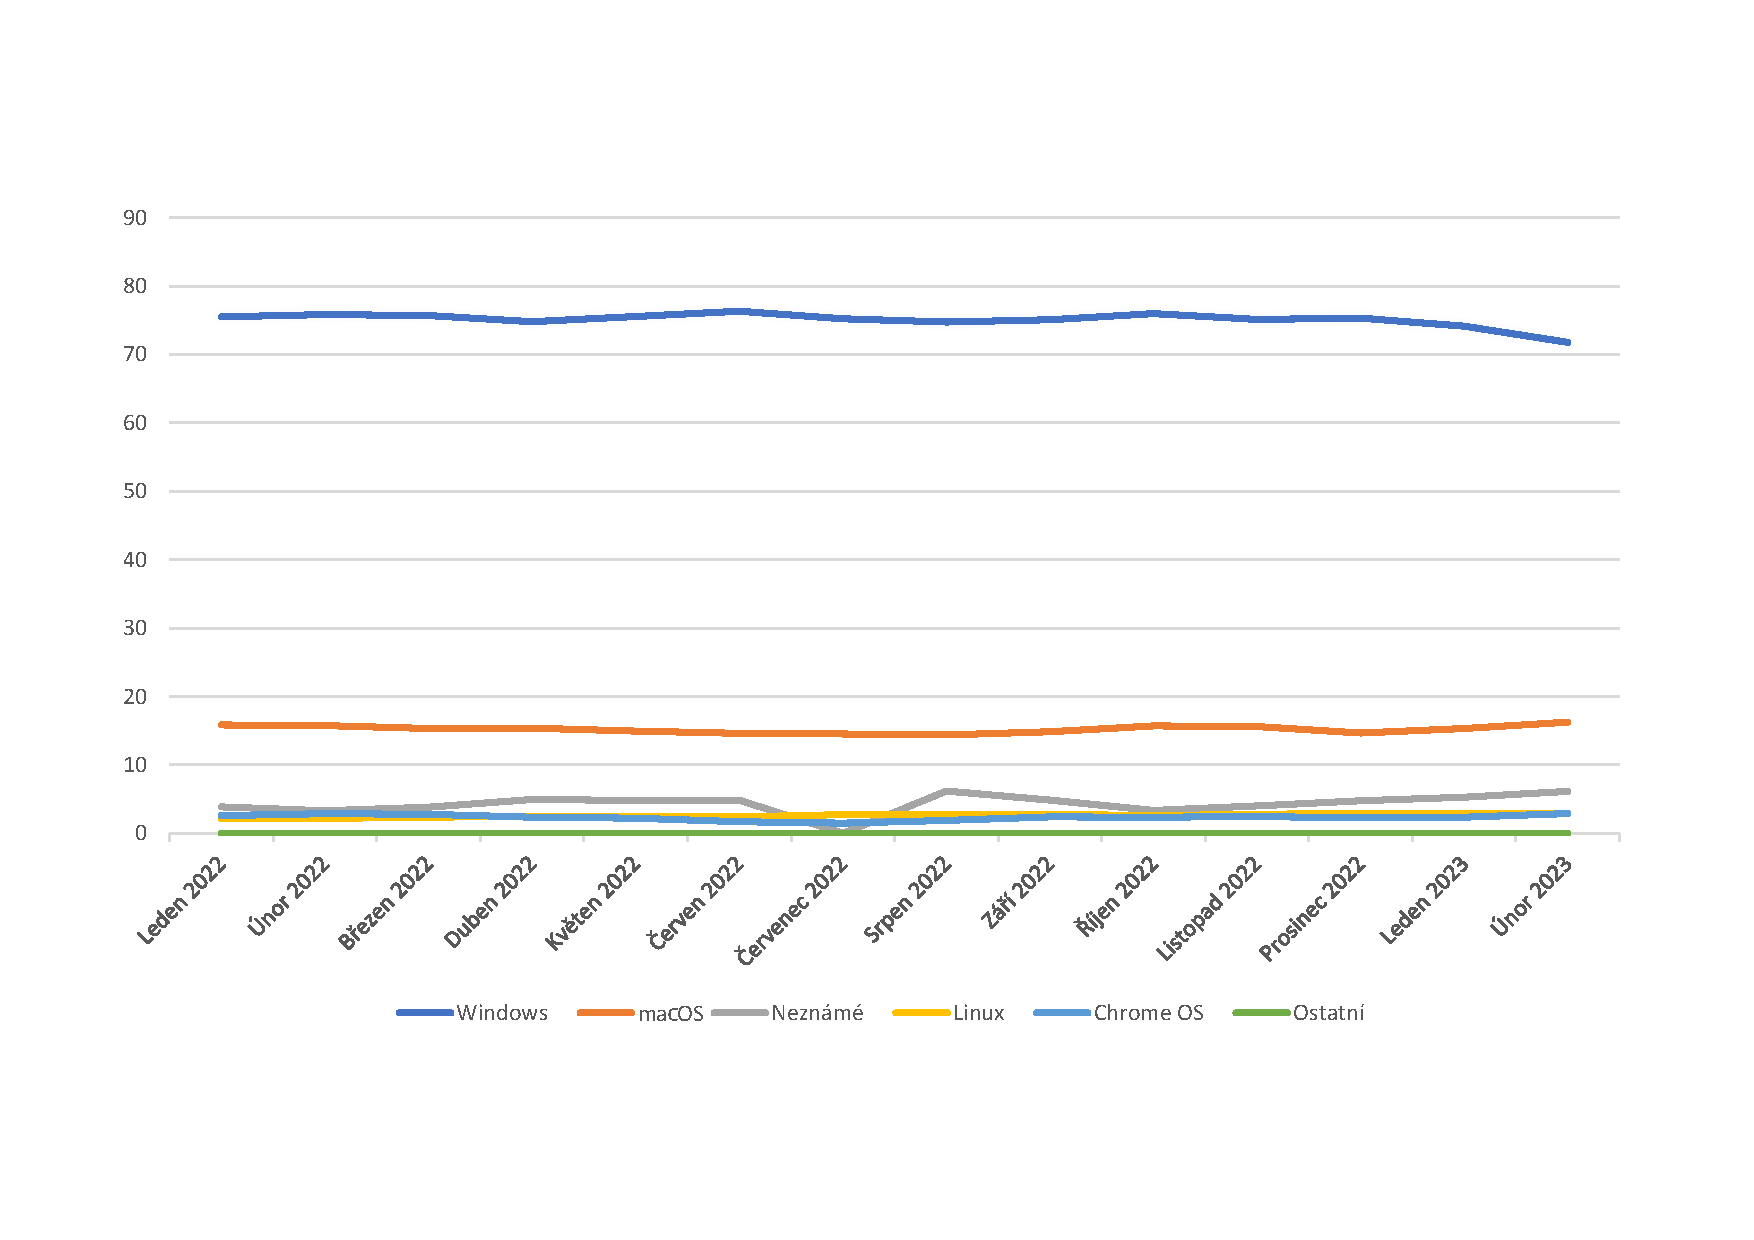
\includegraphics[width=1\textwidth]{Pictures/graf1.pdf}
	\caption{Podíl desktopových OS na trhu (v~\%) \cite{marketshare-desktop-os}}
	\label{fig:MarketshareDesktopOS}
\end{figure}

\subsection{Mobilní aplikace}

Mobilní aplikace jsou takový software, který lze vidět jako kontrast k desktopovým aplikacím. Jsou stavěné pro zařízení s~menšími obrazovkami, bezdrátovým připojením a~napájením z~baterie. V~dnešní době se jedná především o~chytré telefony a~tablety, chytré hodinky nebo např. i~software v~moderních automobilech. Takový software obsahuje různé optimalizace, aby předcházel nadměrnému vybíjení baterie, neboť baterie v~těchto zařízeních nemají vysoké kapacity. Většina těchto zařízení obsahuje dotykové obrazovky pomocí kterých může uživatel komunikovat s~technologií.

Mobilní aplikace jsou stavěné na menší obrazovky, tudíž nemají příliš prostoru na vyobrazování informací - je potřeba zobrazovat pouze ty informace, se kterými uživatele právě pracuje. Toto může být kámen úrazu pro naše využití - vizualizaci onemocnění na mapě ČR. Mapa ČR je vcelku rozsáhlá a~samotná mapa zabere na obrazovce hodně prostoru. Kdybychom chtěli v~aplikaci zobrazovat i~další elementy s~mapou jako např. informace o~zvoleném okrese, dodatečné grafy nebo nastavení, z~obrazovky by se zkrátka stal chaos. Řešením by mohly být chytré tablety, ale tato zařízení mají oproti chytrým telefonům podíl na trhu pouhých 3 až 4 \% \cite{marketshare-mobile-tablet}.

Podobně jako u~desktopových aplikací je nutné aplikaci stavět pro určitý mobilní operační systém neboť tyto systémy nejsou mezi sebou kompatibilní. Mezi nejpoužívanější mobilní OS patří Android společně s~iOS, kde Androidu náleží podíl na trhu kolem 70 \% ze všech mobilních OS \cite{marketshare-mobile-os}.

\begin{figure}
	\centering
	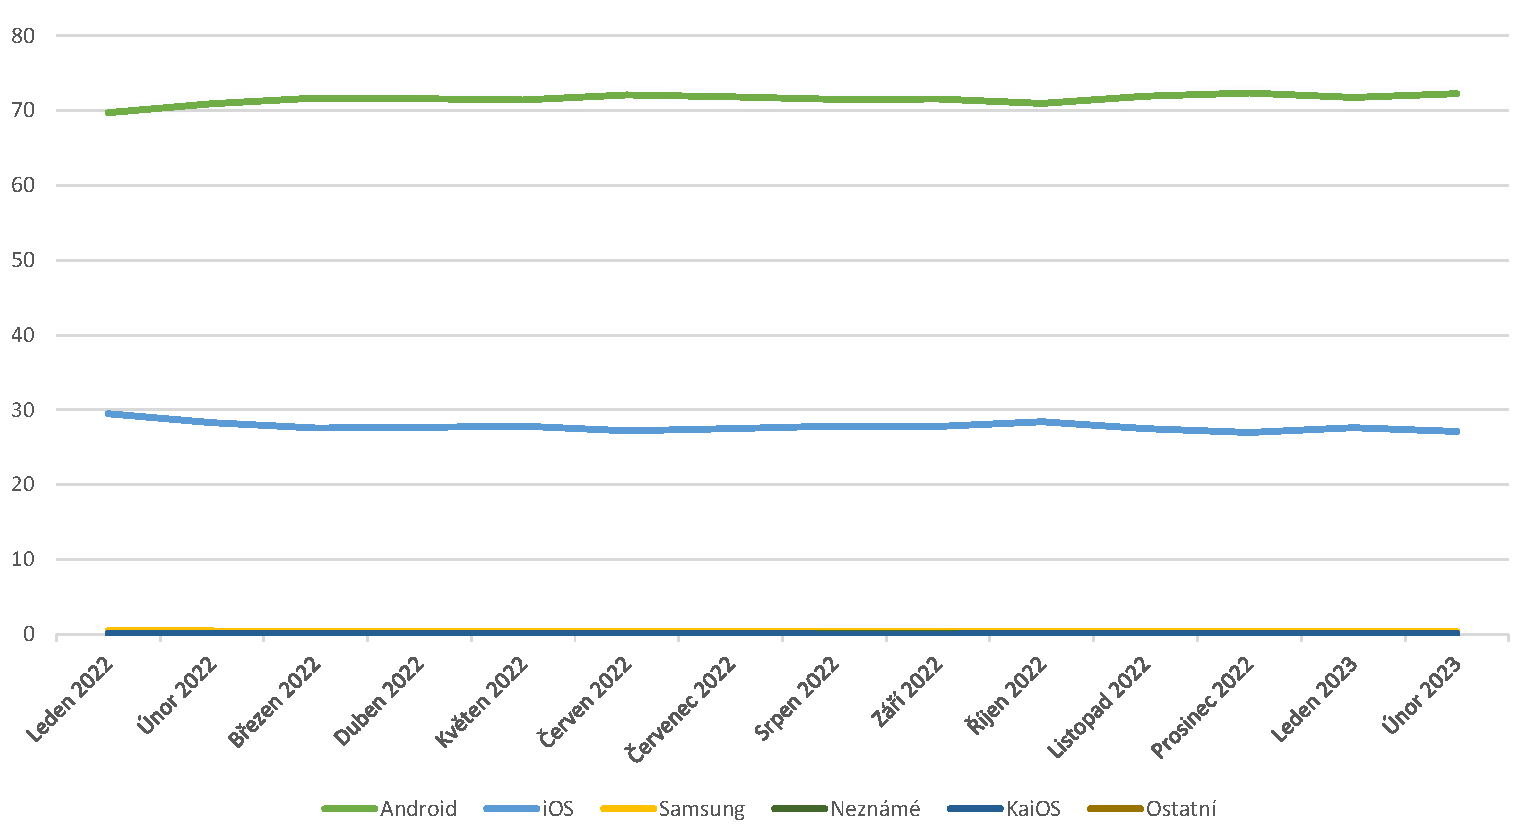
\includegraphics[width=1\textwidth]{Pictures/graf2.pdf}
	\caption{Podíl mobilních OS na trhu (v~\%) \cite{marketshare-mobile-os}}
	\label{fig:MarketshareMobileOS}
\end{figure}


\subsection{Webové aplikace}

Posledním možným řešením je webová aplikace. Webová aplikace je odlišná od desktopových a~mobilních tak, že je uložena na vzdáleném serveru a~uživatelé k~ní přistupují pomocí webového prohlížeče. Webové prohlížeče již bývají součástí operačních systémů, ať už desktopových nebo mobilních. Pro použití aplikace je potřeba mít přístup k~internetu, některé aplikace dokonce vyžadují neustálé připojení po celou dobu používání. 

Většina webových aplikací se skládá ze dvou hlavních částí - frontend a~backend. Frontend je část aplikace, která se zobrazuje uživateli ve webovém prohlížeči. Jedná se o~rozhraní, tlačítka, formuláře apod. Frontend je vytvářen jazyky jako HTML, CSS a~JavaScript. JavaScript se používá k~interakci s~uživatelem a~pro manipulaci obsahu stránky. Backend je taková část aplikace, která je umístěna na serveru a~zajišťuje různé výpočetní nebo datové operace. Důležitou vlastností backendu je, že dokáže zpracovávat požadavky frontendu a~dokáže pracovat s~databází.

Webové aplikace s~sebou nesou důležitou výhodu - jsou multiplatformní, což znamená, že tyto aplikace fungují na široké škále zařízení i~prohlížečů a~není tak potřeba vytvářet několik verzí pro různé systémy. Takové aplikace není třeba nijak lokálně instalovat, jejich aktualizace probíhají na straně serveru, kde jsou aplikace hostovány, takže uživatel vždy používá nejnovější verzi. V~dnešní době je nejvíce používaným webovým prohlížečem Google Chrome, který podporuje mnoho operačních systémů, např. Windows, macOS, Linux, Android nebo iOS. Jeho podíl na trhu přesahuje 65~\% všech webových prohlížečů \cite{marketshare-browser}. Díky rozsáhlé podpoře systémů tohoto prohlížeče lze zajistit kompatibilitu a~stejnou funkčnost na velkém množství zařízení.

Ideální aplikace pro naše využití by byla taková, která by byla snadno přístupná a~jednoduše použitelná na mnoha zařízeních. Po shrnutí různých typů aplikací jsem se rozhodl zvolit zrovna webovou. Webové aplikace mají dnes širokou škálu možností, dokážou stahovat data z~webových API, komunikovat se servery, tvořit grafy nebo i~vizualizovat mapu ČR. Tudíž by webová aplikace měla být schopna splnit to, co po ní v tomto případě vyžadujeme.

\section{Analýza požadavků vybraného řešení}

Když jsme zvolili webovou aplikaci jako vhodnou variantu, je potřeba zvážit a~zanalyzovat její požadavky, aby byla aplikace funkční a~pracovala správně. Pojďme si prvně ukázat jak obecně webové aplikace fungují:

\begin{enumerate}
    \item Uživatel přistoupí k~webové aplikaci prostřednictvím webového prohlížeče - frontend se stáhne z~webového serveru.
    \item Při interakci s~uživatelem (zmáčknutí tlačítka) může frontend zaslat požadavek na backend.
    \item Jakmile je požadavek předán backendu, provede požadovaný úkol - např. vypočte data nebo získá data z~databáze.
    \item Backend odešle zpět odpověď frontendu.
    \item Frontend zobrazí odpověď uživateli v~prohlížeči \cite{frontend-backend}.
\end{enumerate}

\subsection{Webový prohlížeč}

Podle prvního kroku je zcela zřejmé, že aby uživatel přistoupil k~aplikaci, musí použít webový prohlížeč. Budeme předpokládat, že uživatel bude přistupovat ze svého osobního počítače. Na této platformě patří mezi nejznámější prohlížeče Google Chrome a~jiné prohlížeče založené na projektu Chromium (Opera, Microsoft Edge), Mozilla Firefox nebo Safari. Vzhledem k~tomu, že tyto webové prohlížeče používají rozdílná jádra na zobrazování HTML, může výsledná aplikace vypadat na každém prohlížeči mírně jinak. Hlavní rozdíly lze spatřit u~ovládacích prvků (např. posuvníky nebo přepínače), protože každý prohlížeč používá svůj určitý design. Funkčnost aplikace by neměla být nijak ovlivněna.

\subsubsection*{Technologie použité ve webovém prohlížeči}

Každý moderní webový prohlížeč umí pracovat se třemi základními technologiemi, které jsou využité v~téměř každé webové aplikaci. Jedná se o~HTML, CSS a~JavaScript. Na tyto tři technologie se můžeme dívat tímto způsobem: HTML je konstrukce rodinného domu, CSS je dekorace interiéru a~exteriéru a~JavaScript je systém elektřiny, vody a~mnoha dalších funkčních prvků, díky kterým je dům obyvatelný \cite{what-is-html}.

HTML (\emph{Hyper Text Markup Language}) je značkovací jazyk pro vytváření webových stránek. Tento jazyk vyjadřuje jak je strukturovaný webový dokument a~jak by jej měl webový prohlížeč zobrazit. Struktura se skládá z~elementů vyznačené tagy. Elementy se skládají z~otevíracího tagu, obsahu a~uzavíracího tagu. Některé elementy ale mohou být prázdné, to znamená, že nemají uzavírací tag a~ani obsah, ale místo toho obsahují jediný tag, ve kterém mohou mít zdroj nebo odkaz na obsah, který chcete vložit na webovou stránku. Součástí elementu jsou i~atributy, které více definují chování nebo vzhled elementu \cite{google-scholar-html}. Na výsledné HTML stránce kódu \ref{src:HtmlListing} se nachází obrázek, nadpis a~jeden odstavec textu.

\begin{lstlisting}[style=htmlcssjs,label=src:HtmlListing,caption={Příklad HTML kódu}]
<!DOCTYPE html>
<html>
<body>
    <img src="https://www.w3.org/html/logo/badge/html5-badge-h-solo.png" alt="html_logo" >
    <h1> Toto je nadpis dokumentu </h1>
    <p> Zde je odstavec textu. </p>
</body>
</html>
\end{lstlisting}

CSS (\emph{Cascading Style Sheets}) je jazyk definující grafický vzhled HTML elementů ve webovém dokumentu. Pomocí CSS lze definovat vlastnosti (barvy, zarovnání, velikost písma atd.) pro každý element v~dokumentu. Díky tomuto jazyku můžeme styly definovat jednou pro celý dokument a~není třeba je opisovat při opakovaném použití v~dokumentu. Tyto styly se mohou uplatnit i~ve více dokumentech zároveň, např. v~celé webové aplikaci \cite{google-scholar-css}. Příklad CSS kódu, který styluje nadpisy, odstavce a~obrázky, se nachází v~kódu \ref{src:CssListing}. Porovnání webových stránek s~aplikovaným jednoduchým CSS a~bez stylu lze spatřit ve skupině obrázků \ref{fig:subfigures}.

JavaScript je objektově orientovaný programovací jazyk, který lze použít ve webových stránkách. Jedná se o~nezbytnou součást každé webové aplikace, díky které může webová stránka dynamicky měnit svůj obsah. JavaScript nám umožňuje aktualizovat obsah dokumentu, umístit interaktivní prvky, komunikovat se serverem nebo třeba i~vytvářet hry. Obecně díky JavaScriptu mohou získat webové dokumenty logiku a~dokážou být více responzivní a~interaktivní \cite{google-scholar-js}.


\begin{lstlisting}[style=htmlcssjs,label=src:CssListing,caption={Příklad CSS kódu}]
h1 {
    font-family: 'Brush Script MT', cursive;
    font-size: 40px;
    color: red;
    text-decoration: green solid underline;
}
p {
    font-family: 'Courier New', monospace;
    font-size: 20px;
    color: blue;
    background: aqua;
}
img {
    filter: grayscale(1);
}
\end{lstlisting}


\begin{figure}[h]
\centering
\subfloat[HTML kód \ref{src:HtmlListing} bez CSS stylování]{\label{fig:HTMLexampleWithoutCSS}{
\includegraphics[width=0.4\textwidth]{Pictures/html_kod.png}}}\hfill
\subfloat[HTML kód \ref{src:HtmlListing} s CSS kódem \ref{src:CssListing}]{\label{fig:HTMLexampleWithCSS}{
\includegraphics[width=0.4\textwidth]{Pictures/css_kod.png}}}
\caption{Jednoduchá ukázka porovnání CSS stylů}
\label{fig:subfigures}
\end{figure}


\subsection{Webový framework}
\label{sec:webframework}

Framework je softwarová struktura, která pomáhá při vývoji dalších softwarových projektů a~poskytuje podporu při programování. Tyto frameworky mohou obsahovat různé knihovny, podpůrné programy, návrhové vzory nebo ověřené postupy, zkrátka obsahují nástroje, které urychlují vývoj softwaru. Webový aplikační framework je speciální typ frameworku, který se zaměřuje na vývoj webových aplikací a~webových API. Frameworky často poskytují funkční základ, ke kterému můžeme přidat náš kód \cite{what-is-web-framework-geeks}. Použití nějakého webového aplikačního frameworku je nutné pro realizaci naší aplikace. Tyto frameworky dokážou zpracovávat HTTP požadavky, dokážou řídit a~spravovat databázi, mohou zlepšit zabezpečení a~tvořit výstupní data na základě požadavku uživatele \cite{what-is-web-framework-medium}. Příkladem tohoto typu frameworku mohou být např. Django, Ruby on Rails nebo ASP.NET.

\subsubsection*{Django}

Framework, který bude pro tuto práci využit, se jmenuje Django. Django je populární webový open-source framework napsaný v~programovacím jazyce Python. Je vyvinut na základě konceptu DRY (\emph{Don't Repeat Yourself}), který zdůrazňuje důležitost minimalizace duplicitního kódu. Django obsahuje mnoho vestavěných nástrojů jako jsou například správa uživatelů, autentizace a~správa databází. Tento framework je založen na architektuře MTV (\emph{Model-Template-View}), která je hodně podobná architektuře MVC (\emph{Model-View-Controller}). To poskytuje oddělení logiky, uživatelského rozhraní a~datového modelu \cite{django-dry,django-online-dokumentace}. 

Funkce v Djangu, které zpracovávají webové požadavky a~vrací odpovědi, se nazývají zobrazení (\emph{views}) a~jsou uloženy ve \emph{views.py}. Aby Django věděl jakou z~těchto funkcí má spustit, používá URL mapovač v~\emph{urls.py}, který přesměrovává požadavky danému zobrazení podle URL požadavku. Navíc může tento mapovač předat data do zobrazení, která byla obsažena v~URL adrese (např. data formulářů). Django také umí pracovat s~modely (\emph{models.py}). Každý tento model je třída, která se mapuje do jedné databázové tabulky. Na základě těchto modelů Django automaticky vygeneruje API, které umožňuje spravovat (přidávat, upravovat, odstraňovat) záznamy v~databázi. K~zobrazování a~generování stránek a~jejich obsahu využívá tento framework šablony (\emph{templates}). Podle těchto šablon se generují webové stránky a~mohou se naplnit daty z~modelů nebo jiných zdrojů \cite{what-is-django}. Zjednodušený postup zpracování HTTP požadavku Djangem lze vidět na obrázku \ref{fig:DjangoDiagram}.

\begin{figure}
	\centering
	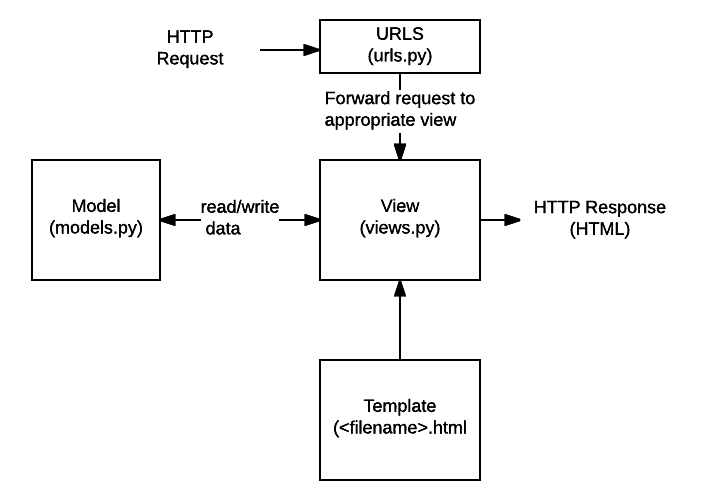
\includegraphics[]{Pictures/django-diagram.png}
	\caption{Postup zpracování HTTP požadavku v Djangu \cite{what-is-django}}
	\label{fig:DjangoDiagram}
\end{figure}

\subsection{Databáze}
\label{sec:DatabaseTheory}

Tato aplikace pracuje s~daty onemocnění covid-19, přístup k~nim nám umožňuje API portálu Onemocnění aktuálně. Vzhledem k~tomu, že je toto API veřejné a~je k~němu teoreticky neomezený přístup, nemusí nám toto API vždy rychle odpovědět. Proto by bylo vhodné mít data uložena lokálně v~backendu. To nám umožní si data libovolně předzpracovat a~díky tomu můžeme urychlit aplikaci. Nejlepší metoda pro ukládání dat by byla pravděpodobně použití databáze. Databáze je z~hlediska IT organizovaná sada strukturovaných informací nebo dat, které jsou uloženy v~elektronické podobě v~počítačovém systému. Tyto databáze ve většině případů používají strukturovaný dotazovací jazyk SQL pro manipulaci samotné databáze a~dat. Databáze obvykle vyžadují správu pomocí systému řízení báze dat (DBMS) \cite{what-is-database-oracle}.

Databázový systém, který je použitý pro tuto aplikaci, se nazývá SQLite. SQLite je relační databázový systém, který se používá pro ukládání dat v~souborech. Jedná se o~open-source software, který je zdarma dostupný pro použití v~komerčních i~nekomerčních projektech. Jeho důležitou vlastností je malá velikost a~nenáročnost. To znamená, že SQLite soubory mohou být velmi malé, často v~rámci jednotek MB, i~přesto, že mohou obsahovat velké množství dat. SQLite podporuje většinu standardních SQL příkazů, což znamená, že se s~ním lze snadno pracovat, pokud máte zkušenosti s~jinými relačními databázovými systémy. SQLite také umožňuje vytváření indexů pro rychlejší vyhledávání dat a~podporuje transakce pro zajištění konzistence dat \cite{what-is-sqlite}.

Jak bylo zmíněno, SQLite pracuje s~jednoduchými databázovými soubory. Pro práci s~těmito soubory bylo vytvořeno mnoho softwaru, mezi takové programy patří např. DB Browser for SQLite. Jedná se o~kvalitní open-source vizuální nástroj pro vytváření, navrhování a~úpravy databázových souborů kompatibilních s~SQLite. Tento program bude použit pro vytvoření databáze a~práci s~ní. Ukázka tohoto programu je na obrázku \ref{fig:SQliteScreenshot}.

Díky své jednoduchosti a~malé velikosti je SQLite ideální pro toto použití, v~tomto případě není třeba používat složitější relační databázové systémy jako např. MySQL.

\begin{figure}
	\centering
	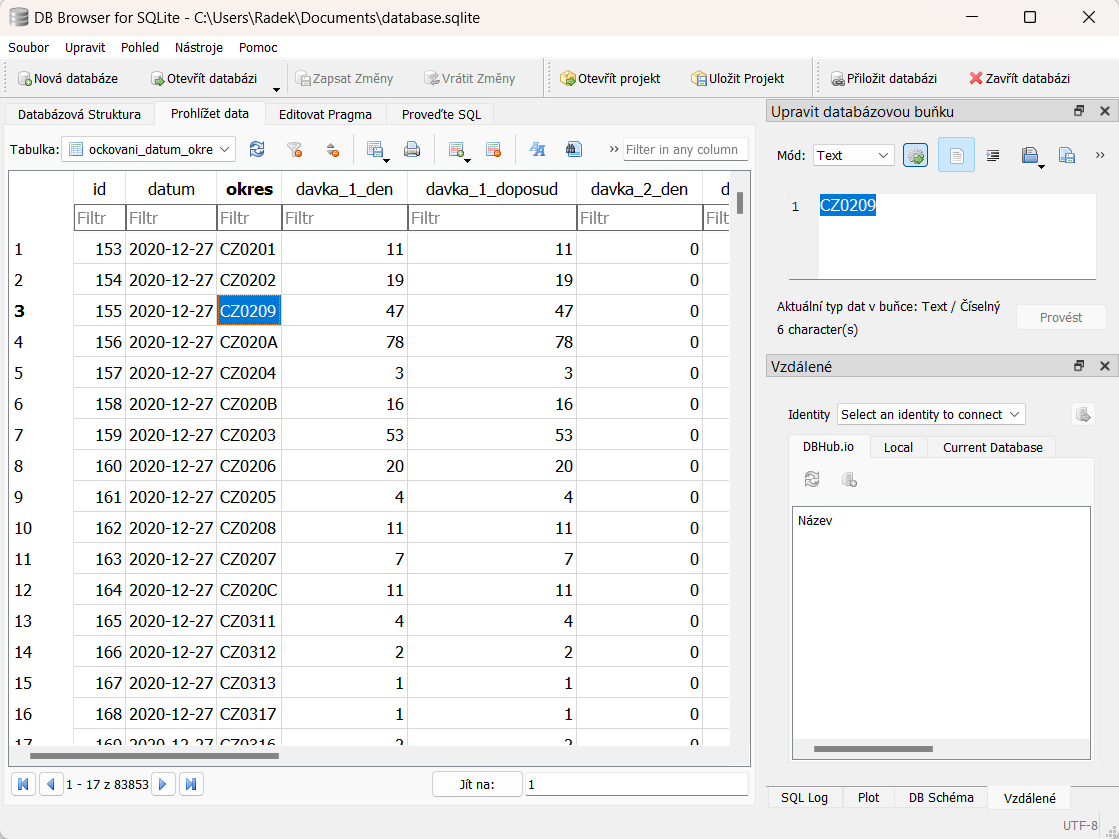
\includegraphics[width=0.8\textwidth]{Pictures/screen_sqlite.png}
	\caption{Program DB Browser for SQLite s~otevřeným databázovým souborem \cite{dbbrowser}}
	\label{fig:SQliteScreenshot}
\end{figure}

\subsection{Způsob vizualizace okresů}
\label{sec:GeoJSON}

Existuje několik způsobů jak vizualizovat územní celky státu na mapě. Byla zvolena možnost vyobrazení pomocí GeoJSONu neboť je tento formát používán v~knihovně, která bude využita pro vytvoření interaktivní mapy.

GeoJSON je formát pro kódování různých geografických datových struktur pomocí JSONu. To umožňuje zakódovat různé geometrické útvary - body, linie, mnohoúhelníky a~další útvary a~dokáže k~nim přidat různé další vlastnosti. Tyto zakódované útvary jsou tzv. GeoJSON objekty. Sady těchto objektů jsou obsaženy v~nadúrovňových objektech \lstinline{FeatureCollection} nebo \lstinline{GeometeryCollection} \cite{google-scholar-geojson}. Každý útvar je definován svým typem a~souřadnicemi na mapě. Ke každému útvaru lze také připsat dodatečné informace, třeba o~jaké místo se jedná.

Pro tvorbu GeoJSON souborů existuje mnoho nástrojů, ve velké většině z~nich se jedná o~webové aplikace. Jedním z~nich je GeoJSON.io \cite{geojson.io}. Tento online nástroj umožňuje nejen vytvářet GeoJSON soubory, ale také dokáže pracovat s~jinými typy souborů a~vyobrazovat je na mapě. Umí pracovat s~formáty jako GPX, CSV, KML nebo samotným GeoJSON \cite{geojson.io}.

Aplikace obsahuje interaktivní mapu s~nástroji kreslení geometrických útvarů. Po dokončení útvaru vám aplikace na pravé straně stránky převede daný útvar do GeoJSONu. Poté stačí kód zkopírovat a~data jsou hotova. Na obrázku \ref{fig:GeoJson.ioScreen} lze vidět aplikaci společně s~vytvořeným kódem pro lokaci Katedrály sv. Víta v~Praze.

\begin{figure}[h]
	\centering
	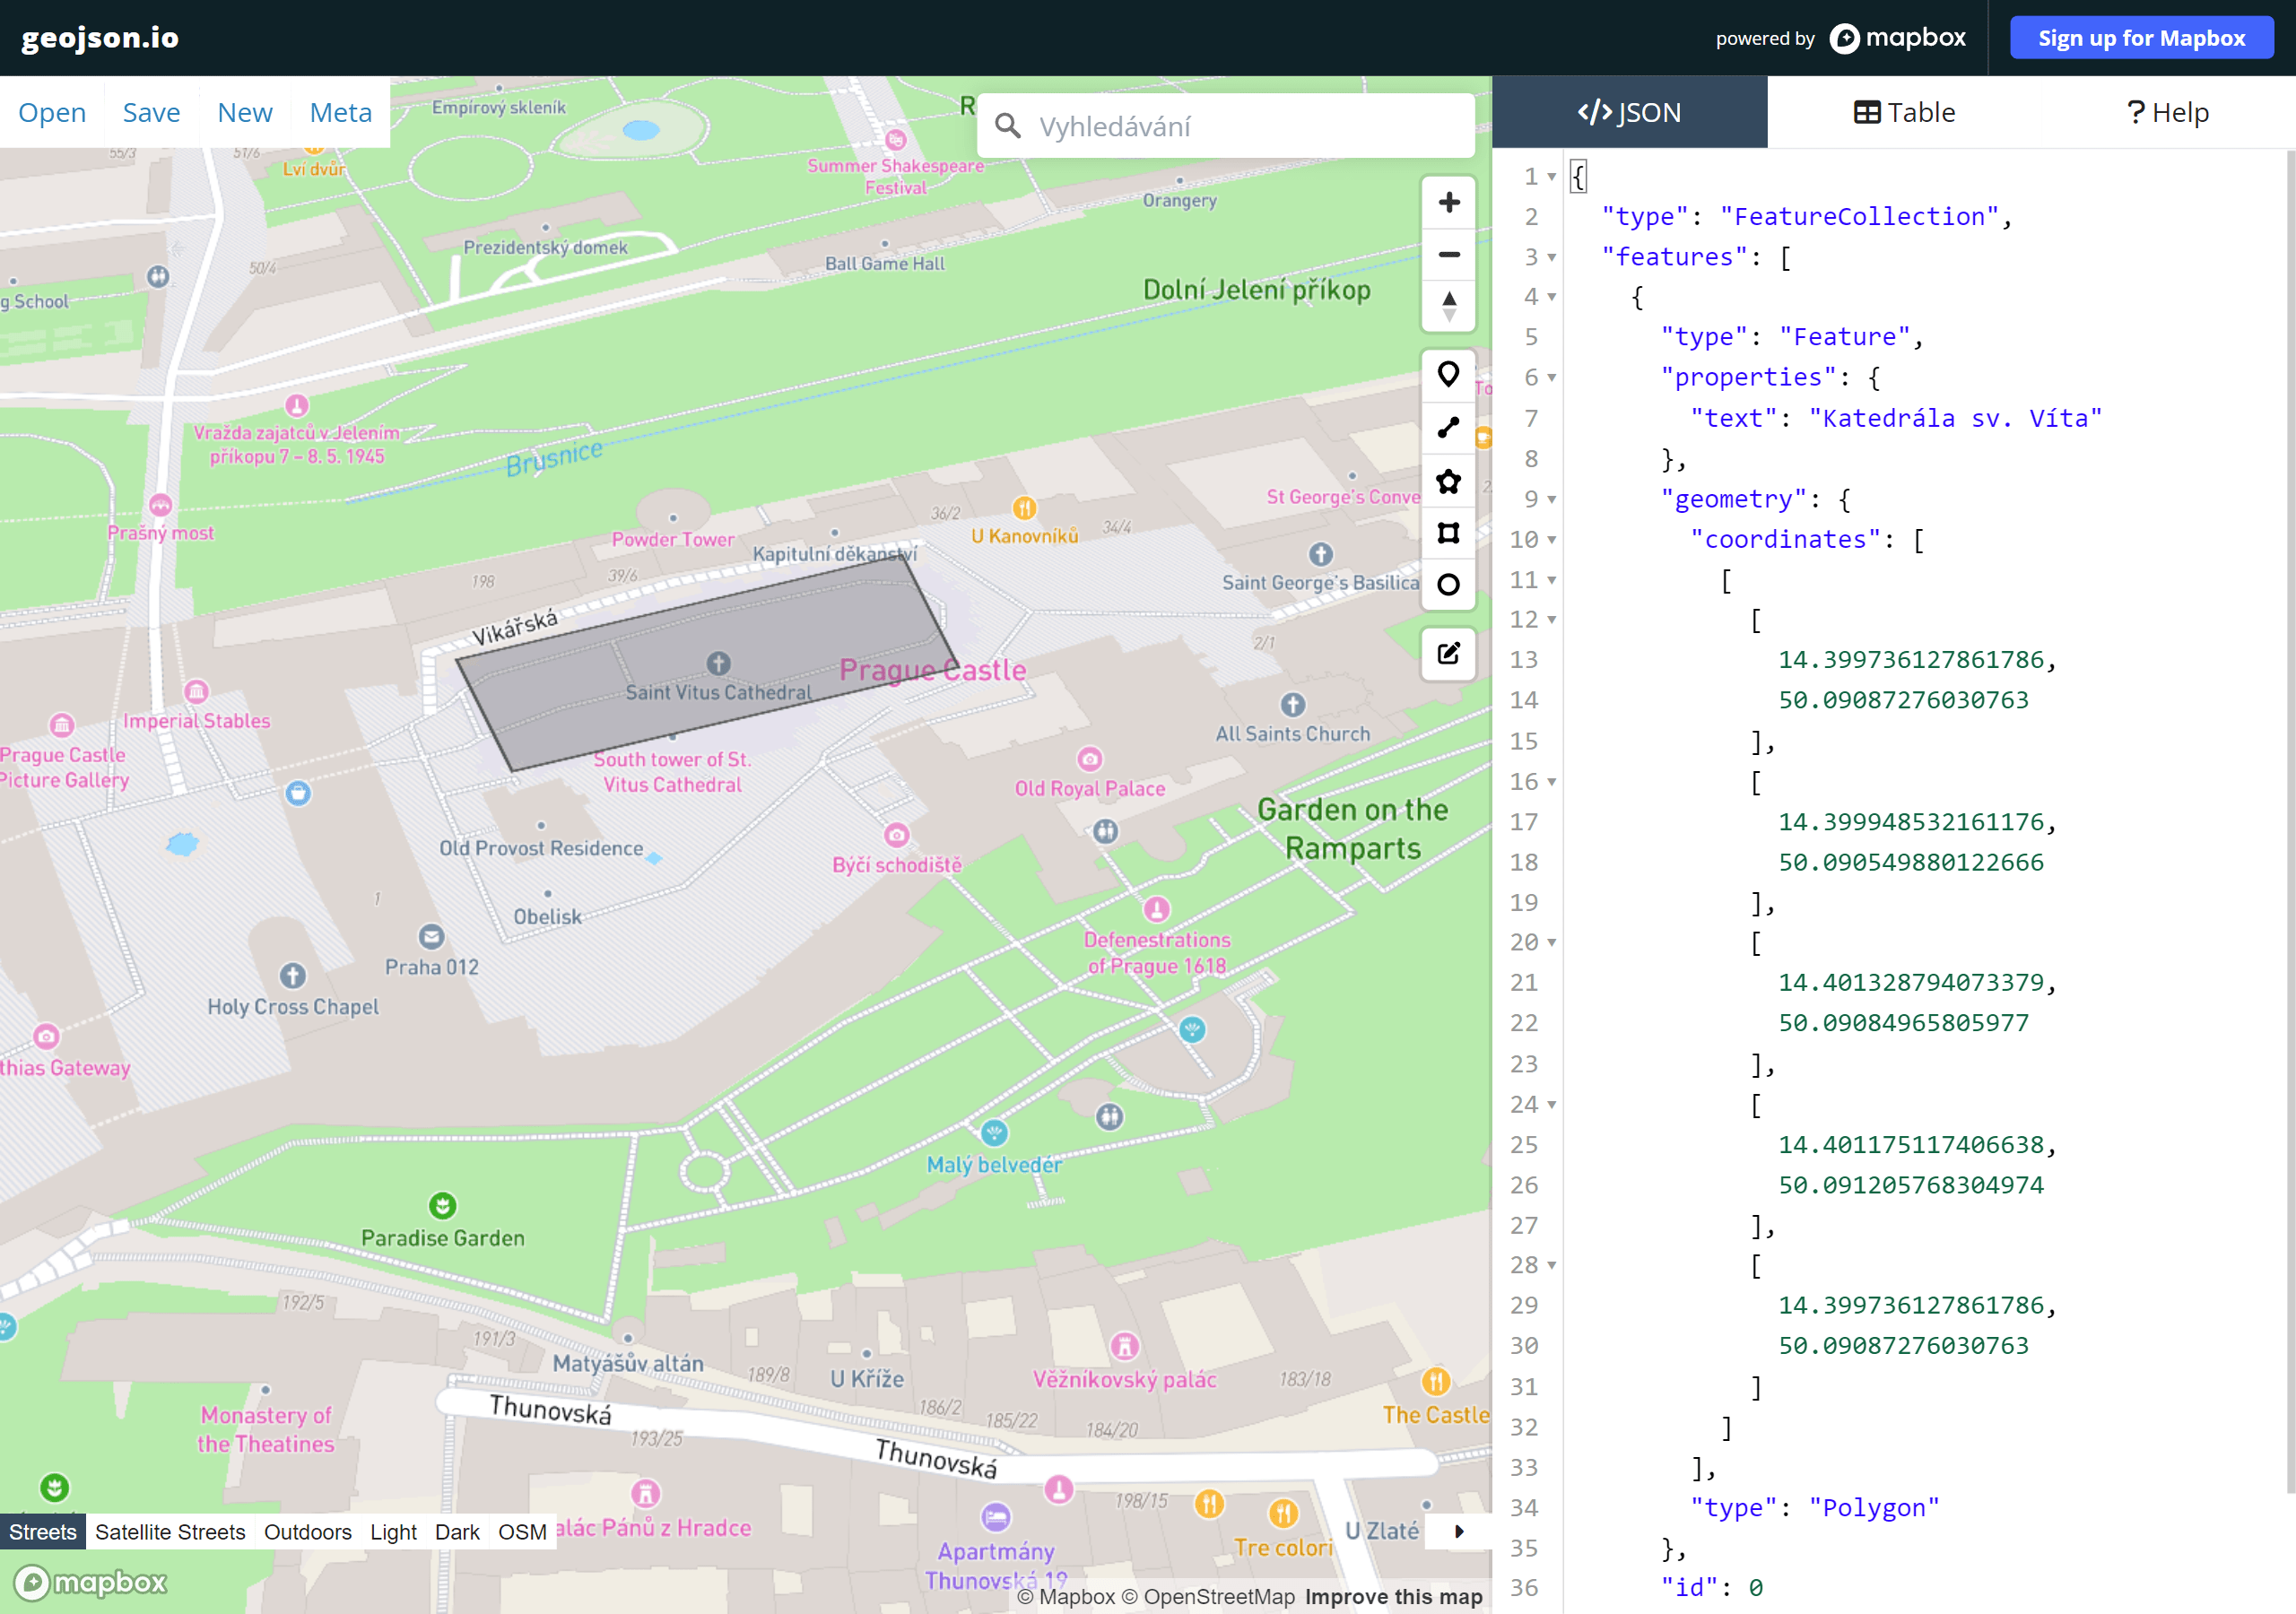
\includegraphics[width=1\textwidth]{Pictures/geojson_screen.png}
	\caption{Práce s~webovou aplikací geojson.io \cite{geojson.io}}
	\label{fig:GeoJson.ioScreen}
\end{figure}